\documentclass[12pt]{article}
\usepackage{graphicx}
\usepackage[margin=1.5in]{geometry}
\usepackage{fullpage}
\usepackage{wrapfig}
\usepackage[colorlinks]{hyperref}
\usepackage{float}

\usepackage{tikz}
\usetikzlibrary{shapes.geometric, arrows}

\tikzstyle{startstop} = [rectangle, rounded corners, minimum width=3cm, minimum height=1cm,text centered, draw=black, fill=red!30]


\tikzstyle{io} = [trapezium, trapezium left angle=70, trapezium right angle=110, minimum width=3cm,,minimum height=1cm,text width=3cm, text centered, draw=black, fill=blue!30]

\tikzstyle{process} = [rectangle, minimum width=3cm,text width=3cm, minimum height=1cm, text centered, draw=black, fill=orange!30]
\tikzstyle{decision} = [diamond, minimum width=3cm,text width=3cm, minimum height=1cm, text centered, draw=black, fill=green!30]

\tikzstyle{arrow} = [thick,->,>=stealth]





\begin{document}




\begin{center}
\textbf{\LARGE  Assignment No.- 6} 
\end{center}

\begin{center}
\textbf{\LARGE ELP - 718 Telecom Software Lab }
\end{center}
\begin{center}

\end{center}
\begin{center}
\textbf{\large  Bhawna Kamra}
\end{center}
\begin{center}
\textbf{\large 2017JTM2187 }
\end{center}
\begin{center}
\textbf{\large Semester-1 }
\end{center}


\begin{center}

\end{center}
\begin{center}

\end{center}






\centering
A report presented for the assignment
Developing logical skills to solve the given problem with the help of basic C.




\begin{center}

\end{center}

\begin{center}

\end{center}



\begin{figure}[H]
\center
\includegraphics[scale=0.5]{images.png}
    
    
\end{figure} 

\begin{center}

\end{center}
\begin{center}

\end{center}

\begin{center}
Bharti School  \\
Telecommunication Technology and Management  \\
IIT DELHI  \\
India  \\

August 2, 2016

\end{center}

  
\newpage
\tableofcontents
\pagebreak
\begin{flushleft}


\section{ Problem statement 1}

\end{flushleft}
\begin{flushleft}
3X3 Numeric Tic-Tac-Toe (Use numbers 1 to 9 instead of X’s and O’s)
One player plays with the odd numbers (1, 3, 5, 7, 9) and other player plays with the even numbers (2,4,6,8). All numbers can be used only once. The player who puts down 15 points in a line wins (sum of 3 numbers). Always Player with odd numbers start the game. Once a line contains two numbers whose sum is 15 or greater, there is no way to complete that line, although filling in the remaining cell might be necessary to complete a different line.
Note – Line can be horizontal, vertical or diagonal

\textbf{Constraints:}
\begin{enumerate}
\item $ 1<=Position<=9$
\item $ 1<=Number<=9 $
\item $1<=Sum<=15$

\end{enumerate}




\end{flushleft}

\begin{flushleft}


\subsection{Terminal:}

\begin{enumerate}

\item Print ‘Welcome to the Game!’.
\item Print whether it is Player 1’s or Player 2’s chance.
\item Get the position and number to be entered from user.
\item Show tic tac toe with data.
\item Continue till the game gets draw or some player wins and show result.
\item Ask user whether to continue for next game or exit.



\end{enumerate}


\end{flushleft}



\begin{flushleft}


\subsection{Structure Chart}
\begin{center}

\end{center}
\end{flushleft}

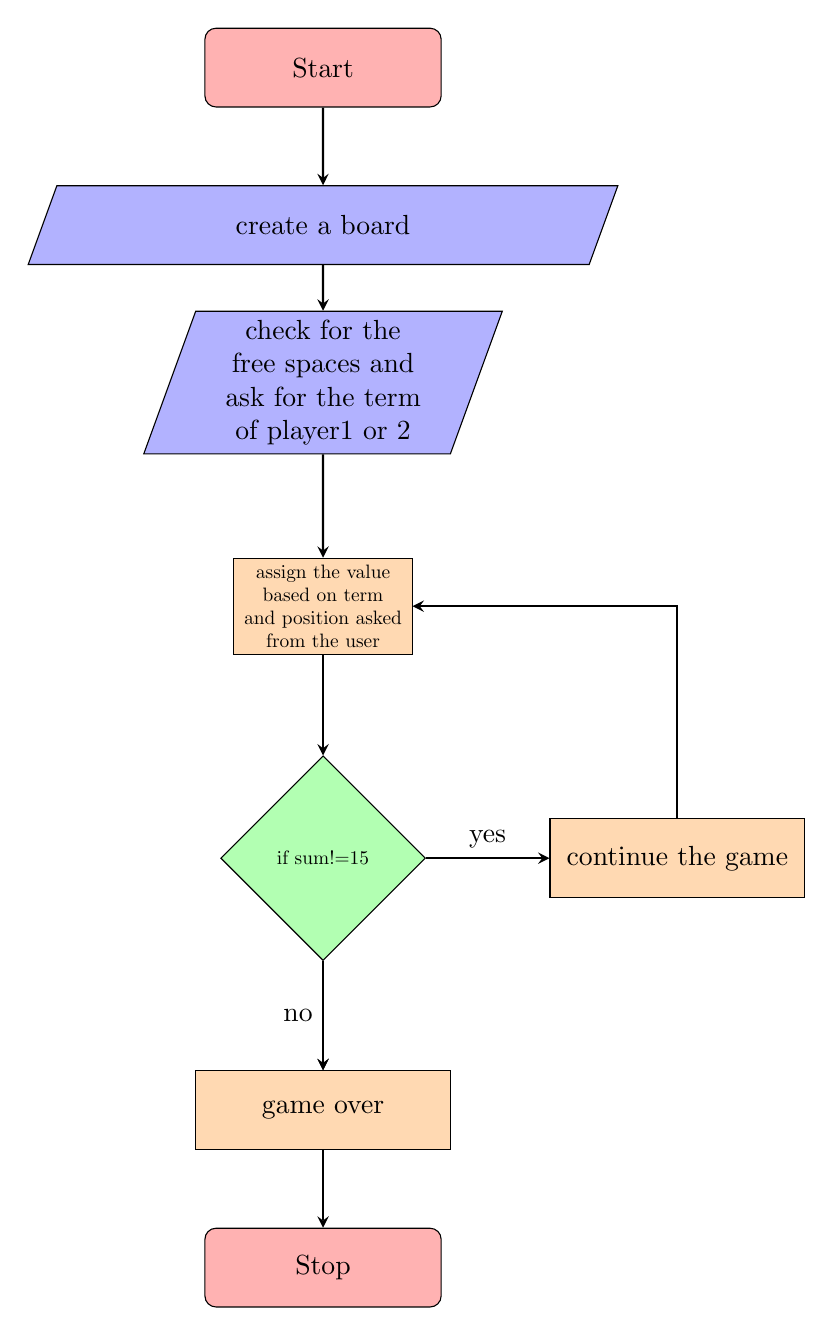
\begin{tikzpicture}[node distance=2cm]

\node (start) [startstop] {Start};

\node (in1) [io, below of=start] {create a board};

\node (in2) [io, below of=in1] {check for the free spaces and ask for the term of player1 or 2};




\node (pro1) [process, below of=in2,scale=0.7,yshift=-1.2 cm] {assign the value based on term and position asked from the user};
\node (dec1) [decision, below of=pro1,yshift=-1.2 cm,scale=0.7] {if sum!=15};
\node (pro2a) [process, right of=dec1,xshift=2.5 cm] {continue the game};


\node (pro2) [process, below of=dec1,yshift=-1.2 cm] {game over};

\node (stop) [startstop , below of=pro2] {Stop};


\draw [arrow] (start) -- (in1);
\draw [arrow] (in1) -- (in2);
\draw [arrow] (in2) -- (pro1);
\draw [arrow] (pro1) -- (dec1);
\draw [arrow] (dec1) -- (pro2);

\draw [arrow] (pro2a) |- (pro1);

\draw [arrow] (pro2) -- (stop);


\draw [arrow] (dec1) -- node[anchor=south] {yes} (pro2a);
\draw [arrow] (dec1) -- node[anchor=east] {no} (pro2);











\end{tikzpicture}
\begin{flushleft}



\subsection{ Output Format}
\begin{flushleft}
Welcome to the Game!
Player 1’s chance
Enter the position and number to be entered: 5,3



Player 2’s chance
Enter the position and number to be entered: 7,4





 






\end{flushleft}



\end{flushleft}







\end{document}
